\chapter{Design and Methodology}

\section{Introduction}

In this section the design and methodology choices involved in this project will be presented. This project consists of five main stages (Figure ~\ref{fig:pipeline}), each of which will be discussed in this chapter. These five stages are:
\begin{itemize}
    \item Data Collection and Filtering: Collecting the data and filtering it so it only contains tweet about hotels posted from Dublin.
    \item Dataset Annotation: Annotating the filtered dataset.
    \item Classification: Training and evaluating multiple supervised machine learning classifiers.
    \item Sentiment Analysis: Analysing the sentiment of the tweets classified as reviews.
    \item Application to Recommender System: Using the sentiment scores produced to re rank the results of the CoRE recommender system.
\end{itemize}

\begin{figure}[h!]
\centering
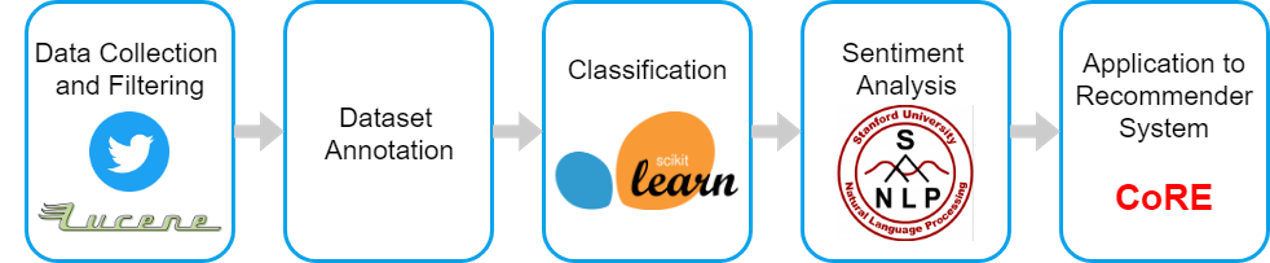
\includegraphics[width=1\textwidth]{project/pipeline.png}
\caption{\label{fig:pipeline} Overview of Project.}
\end{figure}

\section{Data Collection}
The data was collected using the Twitter Streaming API between October 2017 and September 2018. Twitter has a Search API and a Streaming API. The Search API allows you to find historical tweets and the Streaming API allows you to stream real-time tweets.

The data for this project was collected using the Streaming API. A filter was specified so that only tweets posted from within a bounding box of Dublin were returned. A total of 2.5 million tweets were collected.

After inspecting the collection of tweets it was found that although a bounding box had been specified not all tweets were posted from Dublin. A significant amount of tweets had slipped through Twitter's location filter. This meant the first step was to filter the dataset.

\section{Data Filtering}

\subsection*{Geo-tagged Tweets}

All of the tweets in the dataset were Geo-tagged. This meant they all had location data, a specified location from which the tweet was posted. There are two main types of Geo-tagged tweets:
\begin{itemize}
    \item Tweets with a specific latitude/longitude or 'Point' coordinate. These tweets come from GPS enabled devices (Listing ~\ref{lst:pointjson}).
    \item Tweets with a bounding box or Twitter 'Place'. A bounding box is a four-sided geographic area, defined by four points of the form [longitude, latitude]. This defines the general area the tweet was posted from (Listing ~\ref{lst:placejson}).
\end{itemize}

\begin{lstlisting}[caption={Geo-tagged Tweet with Point Coordinate},
captionpos=b,label=lst:pointjson,language=json,firstnumber=1]
"geo": {
    "type": "Point",
    "coordinates": 
        53.28581863,
        -6.11439315
    ]
}
\end{lstlisting}

\begin{lstlisting}[caption={Geo-tagged Tweet with Twitter Place},captionpos=b,label=lst:placejson,language=json,firstnumber=1]
"place": {
  "full_name": "Dun Laoghaire-Rathdown, Ireland",
  "url": "https://api.twitter.com/1.1/geo/id/723427e351a01e72.json",
  "country": "Ireland",
  "place_type": "city",
  "bounding_box": {
    "type": "Polygon",
    "coordinates": [
      [
        [
          -6.282038,
          53.199283
        ],
        [
          -6.282038,
          53.315283
        ],
        [
          -6.066759,
          53.315283
        ],
        [
          -6.066759,
          53.199283
        ]
      ]
    ]
  },
  "country_code": "IE",
  "attributes": {},
  "id": "723427e351a01e72",
  "name": "Dun Laoghaire-Rathdown"
}
\end{lstlisting}

\subsection*{Filtering Out Non-Dublin Tweets}

The first attempt to filter out any non Dublin tweets involved using the 'Point' coordinate of the tweets. The point coordinate of each tweet was compared to the bounding box of Dublin. If it lay inside the box it was kept, otherwise it was filtered out. However, only 7.23\% of the tweets in our collection had a specific 'Point' coordinate. Filtering based on this excluded the majority of the dataset. To address this we instead filtered tweets based on either their 'Point' coordinate or their Twitter 'Place'.

All of the tweets in the collection have a Twitter 'Place' defining the general area that the tweet was posted from. A combination of the Twitter 'Place' and the 'Point' coordinates was used to filter out any non Dublin tweets that had ended up in the dataset. 

\begin{table}[h!]
\caption{Coordinates for Dublin's Bounding Box}
\label{tab:dublinbb}
\begin{tabular}{|l|l|}
\hline
North Latitude  & 53.425210 \\ \hline
South Latitude  & 53.223430 \\ \hline
East Longitude & -6.043924 \\ \hline
West Longitude & -6.447485 \\ \hline
\end{tabular}
\end{table}

A bounding box for the Dublin area was defined (Table ~\ref{tab:dublinbb}). Then tweets with a 'Point' coordinate and tweets with only a Twitter 'Place' were treated differently:
\begin{itemize}
    \item \textbf{Point Coordinates}\newline
    Each tweet with a point coordinate was checked to see if it fell within the defined bounding box for Dublin. If it lay inside the box it was kept, otherwise it was filtered out.
    \item \textbf{Twitter Place}\newline
    Each tweet with a Twitter 'Place' has a bounding box specifying the 'Place'. The centroid of this bounding box was calculated for each tweet. Then the centroid was checked to see if it fell within the defined bounding box for Dublin. If it lay inside the box it was kept, otherwise it was filtered out.
\end{itemize}

The filtered dataset consisted of 1.6 million tweets posted from Dublin between October 2017 and September 2018.

\subsection*{Filter Out Tweets About Hotels}

Now that the dataset had been filtered so it only contained tweets posted from Dublin, the next step was to extract the tweets that mentioned hotels.

A list of the hotels in Dublin was compiled. This included the hotel's name and the hotel's Twitter handle (@hotelname). This list consisted of 0000 hotels and Twitter handles.

The tweets were stored in a Lucene index. A fuzzy search query was used to match the tweets against each of the hotel names and hotel Twitter handles. The fuzzy search query uses a similarity measure that is based on the Damerau-Levenshtein algorithm. The maximum edits option was set to two. This means that strings with a maximum difference of two characters would match. This accounted for misspellings and broadened our search slightly. Higher number of maximum edits were experimented with but we found that too many irrelevant tweets were returned.

This further filtered dataset consisted of 3000 tweets about hotels posted from Dublin between October 2017 and September 2018.

\section{Dataset Annotation}

One major goal of this research was to categorise tweets as review-like tweets, tweets that contain come content and irrelevant tweets. In order to train a classifier to do this a set of tweets had to first be manually annotated. The set of 3000 tweets about hotels in Dublin was annotated. This involved building an annotation webpage where users could view tweets and assign them a label.

\subsection*{Annotation Webpage}

A simple webpage was created in order to annotate the tweets (Figure ~\ref{fig:webpage}). The webpage can be found at \url{http://reviewtweets.epizy.com/}. The text of each tweet was displayed alongside three buttons; review, some content and irrelevant. The annotator could click on the option they thought best described the tweet shown. Once they chose a label, the next tweet would be displayed. 

\begin{figure}[h!]
\centering
\fbox{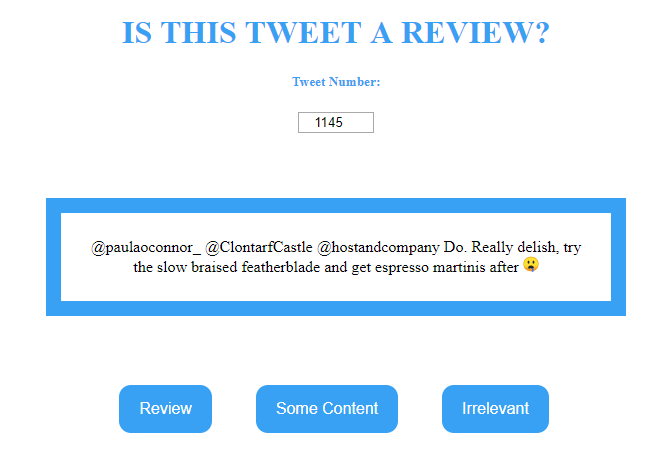
\includegraphics[width=1\textwidth]{project/webpage.PNG}}
\caption{\label{fig:webpage} Webpage for gathering Tweet Annotations.}
\end{figure}

Each time the webpage is loaded a random tweet from the dataset is displayed. The annotator can annotate the tweets incrementally from that random tweet on. This means each annotator will label a different section of the tweets, ensuring all tweets in the collection get annotated evenly.

The following instructions, describing what a review, some content and irrelevant tweet should look like accompanied the webpage:
\begin{itemize}
    \item \textbf{Review} \newline
    The tweet could be considered as a review (of any aspects related to a hotel such as the venue, food, view, swimming pool etc.) for any hotel. Examples would include: \emph{"Amazing view of the Aviva Stadium from my hotel balcony at hotel X"} (positive review), "Room service was awful at hotel Y" (negative review), \emph{"Thank you hotel X for a lovely stay"} (positive review) or \emph{"Had an awful night at hotel Y"} (negative review).
    \item \textbf{Some Content} \newline
    The tweet doesn't look like a review, but it does provide some information related to a hotel, such as the hotel hosts events, information on the menu, information related to accommodation etc. Examples would include: \emph{"Hotel Z serves Tuna salad on Wednesday”} or \emph{“A packed room for the 2018 fashion conference at Hotel X”}.
    \item \textbf{Irrelevant} \newline
    This tweet is completely irrelevant. While perhaps mentioning the name of a hotel, the tweet doesn't give any additional information about that hotel or offer any opinions related to the hotel.
\end{itemize}

In this research we decided to focus solely on the text of the tweets. For this reason all images, videos and URLs were removed from the tweets.

\begin{table}[h!]
\setlength\extrarowheight{5pt}
\begin{tabular}{|l|l|l|l|l|l|}
\hline
    \multicolumn{1}{|l|}{\textbf{Row No.}} & 
    \multicolumn{1}{l|}{\textbf{Tweet ID}} & 
    \multicolumn{1}{l|}{\textbf{Tweet}} & 
    \multicolumn{1}{l|}{\textbf{Review}} & 
    \multicolumn{1}{l|}{\textbf{Content}} & 
    \multicolumn{1}{l|}{\textbf{Irrelevant}} \\ 
\hline
    1 & 00000 & 
    \begin{tabular}[c]{@{}l@{}}
        Creating A Rewarding Experience\\ 
        or CARE, essence of any\\ DoubleTree by Hilton hotels, \\ 
        is in the heart of everything in the\\ 
        Morrison Hotel! \#CARE \\
        \#DoubleTree \#dublincity \\ 
        \#brandculture
    \end{tabular} & 0 & 0 & 0 \\ 
\hline
    2 & 00000 & 
    \begin{tabular}[c]{@{}l@{}}
        @bfitzsimons @doubletree \\
        @DTHydePark Oohh. \\
        Impressed!
    \end{tabular} & 0 & 0 & 0 \\ 
\hline
    3 & 00000 & 
    \begin{tabular}[c]{@{}l@{}}
        SlowMo Training \\ 
        \#EliteFest2018 @ The \\ 
        Morrison, a DoubleTree \\ 
        by Hilton Hotel
    \end{tabular} & 0 & 0 & 0 \\ 
\hline
    4 & 00000 & 
    \begin{tabular}[c]{@{}l@{}}
        Drinking a Heineken by \\ 
        @heineken at @doubletree —
    \end{tabular} & 0 & 0 & 0 \\ 
\hline
\end{tabular}
\caption{Sample of tweets from SQL table}
\label{Table:TweetAnnotation}
\end{table}

The tweets were stored in an SQL table (Table ~\ref{Table:TweetAnnotation}) linked to the webpage, along with a count of the number of times the tweet had been labelled as a review, some content and irrelevant. Each time a user chooses a label the corresponding value in the database is incremented. The final label of a tweet is determined by calculating which label had the maximum number of votes. 

The annotation webpage was circulated to friends, family and members of the Adapt research centre to gather annotations.

\section{Tweet Classification}

The annotated set of tweets was used to train a series of twelve classifiers. Six different feature representations were used. These classifiers were implemented using Python's scikit learn. An 80:20, train test split was used for the data.

\subsection*{Decision Tree}

\subsection*{Random Forest}

\subsection*{Multi Layer Perceptron}

\subsection*{Support Vector Machine}

\subsection*{Logistic Regression}

\subsection*{K Nearest Neighbours}

\subsection*{Gaussian Process}

\subsection*{Adaboost}

\subsection*{Gaussian Naive Bayes}

\subsection*{Bernoulli Naive Bayes}

\subsection*{Quadratic Discriminant Analysis}

\subsection*{Linear Discriminant Analysis}


\section{Sentiment Analysis}

\subsection*{The Stanford Sentiment Analyser}
%Limitations - data it was trained on etc.
\subsection*{Normalising the Sentiment Scores}

\section{CoRE Recommender System}

The sentiment scores produced by the Stanford Sentiment Analyser were used to re rank the list of hotel recommendations produced by the CoRE recommender system.
